% Chapter 1

\chapter{Revue bibliographique} % Main chapter title
\label{Chapter2} % For referencing the chapter elsewhere, use \ref{Chapter1}
%\minitoclt
%\bigbreak
\section{Le bananier}
\subsection{Origine}
\noindent{Originaire du Sud-est asiatique, la banane plantain est retrouvée principalement de l'Inde à la Polynésie (\cite{lassoudiere2010histoire}). Elle est le fruit d'une géante plante de la famille des Musaceae, le bananier plantain. Son centre de diversification semble être la Malaisie ou l’Indonésie (\cite{daniells2001musalogue}).}

\noindent{Le bananier est apparu pour la première fois en Afrique  près de Zanzibar (Tanzanie, Afrique de l’Est) ou le Madagascar (\cite{raemaekers2001agriculture}). En Amérique, son  implantation à commencer d’abord par la République Dominicaine en 1516 par des plants provenant des Iles Canaries et s’est poursuivie vers l’Amérique centrale et du Sud grâce à la migration et aux  échanges de matériels végétaux, ce qui a permis l’introduction du bananier sur tous les continents dans des zones agro-écologiques très différentes (\cite{lassoudiere2007bananier}).}

\subsection{Culture}
\noindent{Principalement produite en Afrique et en Amérique du Sud, les bananiers se multiplient de manière asexuée en produisant des rejets, jeunes plants qui se forment au pied de la plante mère (\href{https://jardinage.ooreka.fr/astuce/voir/499947/banane-plantain}{Oreka}).\\
En production, les jeunes bananiers sont souvent issus de culture in vitro afin d'éliminer les parasites et obtenir des plants sains. En effet, le bananier est principalement sensible aux nématodes, champignons et charançons (\href{https://jardinage.ooreka.fr/astuce/voir/499947/banane-plantain}{Oreka}).\\
La récolte des régimes de banane se fait généralement en moins d'un an après culture .

Avant la culture, la préparation de terrain passe par le défrichement, l’abattage systématique de tous les arbres, le tronçonnage et l’andainage, le piquetage et la trouaison (\href{https://jardinage.ooreka.fr/astuce/voir/499947/banane-plantain}{Oreka}).
}
\subsubsection{Le piquetage de la parcelle :}
\noindent{Le piquetage variant selon les variétés de plantes, le degré de fertilité du sol et des systèmes de culture, consiste à matérialiser les emplacement pour la trouaison avec les piquets.\\
\begin{itemize}
	[label=$\bullet$, leftmargin=1cm, parsep=0cm, itemsep=0cm, topsep=0cm ]
	\item En culture pure, les écartements entre plants pour une densité de 1550 plants par hectare selon (\cite{agricam2018}) sont  3 m x 2 m (3 m entre les lignes et 2 m entre les plants) ou de 3,2 m x 2 m. En ligne double ou jumelée (1,8 x 2 m x 3,6 m), on a une densité de 742 plants par hectare. 
	\item  En culture associé, les écartements sont de 4 m x 4 m, soit 525 plants/ha et permet d’exploiter les espaces entre les pieds de bananier au premier cycle et de construire ensuite la plante à 4 porteurs au second cycle. Les écartements de 4 m x 2 m soit 1250 plants/ha permettent de cultiver d’autres cultures vivrières comme le maïs de manière permanente entre les lignes de bananier plantain (\cite{agricam2018}).
\end{itemize}

}

\subsubsection{La trouaison :}
\noindent{Elle consiste à creuser des trous à l'emplacement des futurs bananiers, là où les piquets ont été plantés. Selon \cite{agricam2018}, la trouaison doit se faire peu de temps avant la mise en terre des rejets pour éviter le remplissage des trous en cas de pluies importantes. Pendant la trouaison, les couches de terre de surface plus noire et riche en matière, et celle de profondeur généralement plus rouge,  devront être maintenues séparément.\\
Les dimensions de 40 cm x 40 cm x 40 cm sont recommandées pour les rejets baïonnettes
ou les PIF. Celles de 50 cm x 50 cm sont conseillées pour les souches à rejets ou à œilleton.}
\begin{figure}
	\centering
	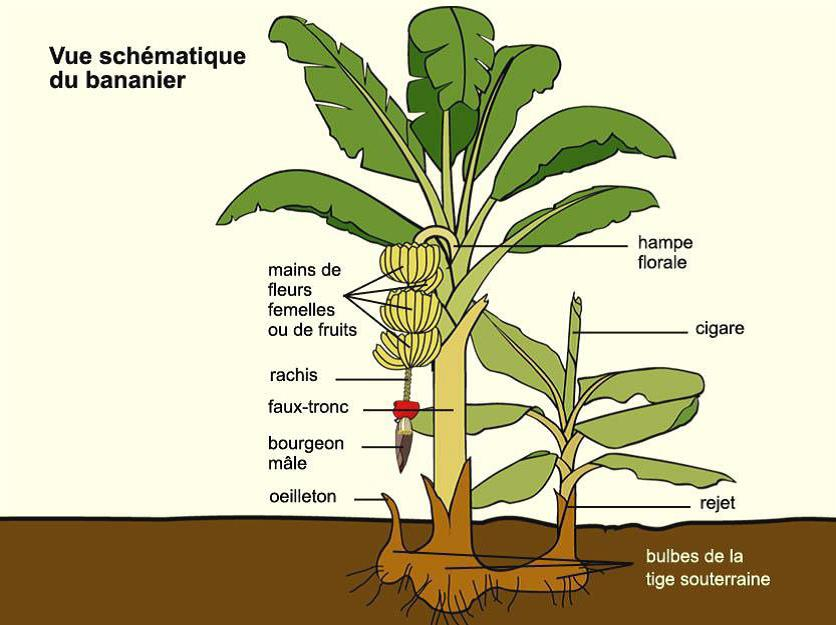
\includegraphics[scale=0.5]{banane}
	\captionof{figure}{Vue schématique d’un bananier à sa fructification et de ses rejets d’après  \cite{champion1967notes}}
\end{figure}

\section{Ravageurs}
\noindent{Parmi les principaux ravageurs des bananiers, se trouvent les nématodes pouvant provoquer des dégâts significatifs selon le milieu et le lieu géographique (\cite{gowen1990nematode}). Le nématode \textit{Radopholus similis} est le plus répandu (\cite{sarh1996nematode}). \textit{Pratylenchus coffeae} et \textit{Pratylenchus goodeyi} provoquent autant de dégâts mais sont moins répandus et relativement peu fréquents sur les bananiers (\cite{bridge1997nematode}). Tous ces nématodes ont un impact sur la production de bananes dans les tropiques alors que le nématode à spirale, Helicotylenchus multicinctus, provoque plus de dégâts dans la zone subtropicale (\cite{mcsorley1986nematological}). Le charançon, \textit{C. sordidus}, est l’insecte qui est le plus répandu et a le plus grand impact sur les bananiers (\cite{gold2001biology}).
}
\subsection{Lutte contre les charançons}
\subsubsection{Lutte chimique}
\noindent{Les pesticides sont d'un grand secours. Leur utilisation a été forte entre 1950 et 1986, les pays en développement utilisant le quart de tous les pesticides consommés dans le monde. Toutefois, un emploi incorrect et excessif de ces produits peut contaminer aussi bien les denrées alimentaires que l'environnement et, dans certains cas, nuire à la santé des agriculteurs (\cite{fao1996insecte}).}

\noindent{Jusqu'aux années 90, la principale technique de lutte contre le charançon était chimique. On retrouvait l'utilisation des fongicides et autres. Aux Antilles Françaises, le chlordécone, pesticide organochloré, était le plus utilisé (\cite{vilardebo1974chlordecone}), avant son interdiciton en 1993 du fait de sa toxicité et de sa forte persistence.}

\subsubsection{Piégeage de masse}
\noindent{Le piégeage de masse consistant à placer des pièges à phéromones dans les bordures des parcelles parcelles afin de limiter la contamination des parcelles avoisinantes (\cite{rhino2010effect}) est aussi un moyen de lutte contre les ravageurs mais, le rayon d'action des pièges et les facteurs influençant l'efficacité du piégeage sont encore méconnus et nécessitent des études approfondies afin d'optimiser la disposition spatiale des pièges à l'échelle de la parcelle, voire du réseau de parcelles.}

\noindent{Face aux pollutions graves liées à la lutte chimique , la résistance des ravageurs à ces méthodes de luttes et la non maîtrise des facteurs influençant l'efficacité du piégeage il urge de trouver de trouver une méthode alternative naturelles de lutte contre les ravageurs.}

\subsubsection{Système de lutte par un prédateur}
\noindent{Les agroécosystèmes diversifiés fournissent de nombreux services à l’homme dont la régulation biologique. L’association des cultures est une pratique agricole qui favorise la diversité des plantes dans les agroécosystèmes, fournit des ressources alimentaires alternatives et structure les communautés des arthropodes. Elle favorise les prédateurs généralistes pour la régulation biologique des ravageurs (\cite{dassou2014effet}).
}

\noindent{La régulation des charançons par contrôle biologique a fait l’objet de plusieurs études (\cite{gold2000biology}, \cite{collard2018spatial}, \cite{dassou2014effet}), bien que rare sont celles qui portent sur le Bénin}

\noindent{Les études sont menées, sur les ennemis naturels du charançon \textit{C. sordidus} afin d’identifier leur efficacité. Les ennemis naturels de \textit{C. sordidus} sont les arthropodes, les nématodes entomopathogènes, ainsi que des champignons entomopathogènes (\cite{gold2000biology}). Plusieurs coléoptères prédateurs qui se nourrissent des  larves du charançon ont été identifiés dans son aire d’origine, l’Asie du Sud – Est. Toutefois des difficultés subsistent pour introduire ses ennemis naturels dans d’autres zones de production (\cite{gold2000biology}). Par contre, l’utilisation des fourmis \textit{myrmicines Tetramorium guinense} et \textit{Pheidole megacephala} dans la lutte contre le charançon \textit{C. sordidus} dans les plantations de Cuba ont connu une efficacité (\cite{gold2000biology}). Les adultes et les larves du charançon dans les champs sont attaqués par les nématodes \textit{entomopathogènes Steinerma et Heterorhabditis spp}., mais ne sont efficaces qu’en fortes densités du charançon.
	
Certaines espèces de fourmis sont connues pour être responsables d’une régulation des populations de \textit{C. sordidus} (\cite{abera2007composition, abera2008experimental}; \cite{gold2001biology}), des taux de prédation
pouvant aller jusqu’à 70\%, comme il a été constaté à Cuba (\cite{perfecto1998deployment}). Les fourmis du genre \textit{Pheidole} ainsi que l’espèce \textit{Ondotomachus troglodytes} sont capables d’extraire naturellement des œufs de charançons dans les bananiers. Il a été également observé à plusieurs reprises des fourmis \textit{Pheidole} s’attaquant à des charançons adultes et les ramenant à leur nid (observation personnelle lors de la collecte des données)

De même, le \textit{dermaptère E. caraibe}, prédateur généraliste des bananeraies de la Martinique, a été testé contre les charançons du bananier (\cite{collard2018spatial}). Il a été constaté que l’abondance et l’activité des \textit{dermaptères} semblaient dépendre fortement des types d’habitats : les résidus de bananiers apparaissant particulièrement plus favorables aux \textit{dermaptères} que le sol nu(\cite{collard2018spatial}).}

\noindent{Afin d’étudier le rôle de la biodiversité, il est important de déterminer quelles sont les cultures présentes dans un écosystème donné et les relations entre elles. Nous étudierons ici l'association de la culture de maïs dans les bananeraies de Toffo}

\section{Modélisation et agroécologie}
\noindent{Il existe différents types de modèles en écologie, chacun ayant des avantages et des inconvénients. Les modèles les plus classiques sont des modèles agrégés, basées sur des équations différentielles ordinaires (EDO) ou partielles (EDP). Ces équations relient l’état d’un système à un instant t à des instants antérieurs. L’état du système est défini par une ou plusieurs variables quantitatives, parmi lesquelles des variables agrégées qui représentent le comportement d’un groupe d’individus, comme la biomasse ou le nombre d’individus (\cite{holt1977predation}; \cite{watson2015exploring}). Les équations de Lotka-Volterra ont été mobilisées pour étudier l’interaction du proie-prédateur dans le cadre du contrôle biologique des ravageurs. Le modèle macro est définie par les équations suivantes :
}

\begin{equation}
	\left\lbrace\begin{aligned}
		\dfrac{dx(t)}{dt}	& = x^{'}(t) = \dot{x} = ax(t)-bx(t)y(t)		\\
		\dfrac{dy(t)}{dt}	& = y^{'}(t) = \dot{y} = -cx(t)-bx(t)y(t)
	\end{aligned}\right.
\end{equation}
$$\systeme{\frac{dx(t)}{dt} = x^{'}(t) = \dot{x} = ax(t)-bx(t)y(t),,\frac{dy(t)}{dt} = y^{'}(t) = \dot{y} = -cx(t)-bx(t)y(t)}$$


\noindent{$x :$ nombre de proies\\
	$y : $ nombre de prédateurs\\
	$dx(t)/dt :$ variation du nombre de proies dans le temps\\
	$dy(t)/dt :$ variation du nombre de proies dans le temps\\
	$a :$ taux de natalité des proies\\
	$c :$ taux de mortalité des prédateurs\\
	$b :$ taux de mortalité des proies lié à la prédation\\
	$d :$ taux de natalité des prédateurs lié à la consommation de proies.\\
}

\noindent{Ces approches peuvent aussi représenter l’espace de manière explicite, où les déplacements des individus ou de leur biomasse sont assimilés à des processus de diffusion (\cite{okubo1980diffusion}; \cite{corbett1993role}; \cite{vinatier2013explaining}).
}

\noindent{De multiples arthropodes peuvent envahir une bananeraie grâce aux cultures associées. Un modèle spatialement explicite permettrait de prendre en compte l'effet des différents arthropodes rencontrés sur les bioagresseurs.\\
Les modèles individu- ou agent-centrés (IBM ou ABM) sont des approches de résolution de problème ascendantes (« bottom-up ») dans lesquels chaque entité du système est représentée par un individu se comportant de manière indépendante des autres (\cite{fachada2015towards}). Nécessitant une implémentation informatique, ce type de modèle est apparu après les travaux de \cite{schelling1969models}. Suite à l’augmentation de la puissance des ordinateurs (\cite{grimm2013individual}), le modèle s'est généralisé à partir de quatre courants de recherche différents : l’écologie, l’informatique et l’ingénierie, les sciences cognitives et les sciences sociales (\cite{tang2010agent})}

\noindent{Le développement d’un modèle de simulation de l’épidémiologie de \textit{C. sordidus}, combiné avec des modèles de croissance végétale a permis d’améliorer l’arrangement spatial des parcelles et les stratégies de piégeage, en lien avec les mouvements du ravageur et leur dépendance à la qualité de l’habitat travers le modèle COSMOS (\cite{vinatier2010dynamique}).\\
Le modèle développé est un modèle individu centré multi-agent. La création d'un système multi-agents consiste à reproduire un monde artificiel qui ressemble au monde observé - c'est-à-dire qu'il est composé de différents acteurs - à des fins expérimentales. Chaque agent est représenté comme une entité informatisée indépendante capable d'agir localement en réponse à des stimuli ou à la  communication avec d'autres agents.}

\section{Modèle spatialement explicit COSMOS}
\noindent{Le modèle COSMOS, vise à simuler l'épidémiologie spatiale de \textit{C. sordidus} à long terme en décrivant la dynamique de sa population et l'infestation des plantes hôtes qui en résulte. Le modèle considère tous les stades de l'insecte simultanément et suppose qu'il existe des variations individuelles de comportement en fonction de chaque stade de développement. Le modèle fonctionne selon l’hypothèse que la distribution des populations et des attaques de C. sordidus dans les champs de bananiers peut être modélisée selon des règles épidémiologiques identifiées au niveau individuel et calibrées à partir de la littérature. Le modèle COSMOS, comme le modèle SIMBA-NEM , centré sur les nematodes et le modèle SIMBA-CC sur les plantes de couvertures (\cite{tixier2008simba}; \cite{tixier2004simba}), vise à combler le fossé entre l'écologie comportementale individuelle et la dynamique des populations (\cite{deangelis1994individual}).  Il a été validé en comparant les sorties du modèle avec les données de terrain. Enfin, COSMOS a été utilisé pour tester comment les schémas de plantation et l'hétérogénéité spatiale des stades de la plante, résultant de la variabilité de l'apparition des drageons au cours des cycles de culture, pouvaient modifier le temps nécessaire à la colonisation de l'ensemble de la parcelle et le niveau des dégâts pendant trois cycles de culture, lorsque la population initiale de charançons était distribuée le long d'un côté de la plantation.}


%---------------------------------------------------------------------------------------

% Define some commands to keep the formatting separated from the content
\newcommand{\keyword}[1]{\textbf{#1}}
\newcommand{\tabhead}[1]{\textbf{#1}}
\newcommand{\code}[1]{\texttt{#1}}
\newcommand{\file}[1]{\texttt{\bfseries#1}}
\newcommand{\option}[1]{\texttt{\itshape#1}}

%---------------------------------------------------------------------------------------

